\documentclass{tufte-handout}\usepackage[]{graphicx}\usepackage[]{xcolor}
% maxwidth is the original width if it is less than linewidth
% otherwise use linewidth (to make sure the graphics do not exceed the margin)
\makeatletter
\def\maxwidth{ %
  \ifdim\Gin@nat@width>\linewidth
    \linewidth
  \else
    \Gin@nat@width
  \fi
}
\makeatother

\definecolor{fgcolor}{rgb}{0.345, 0.345, 0.345}
\newcommand{\hlnum}[1]{\textcolor[rgb]{0.686,0.059,0.569}{#1}}%
\newcommand{\hlstr}[1]{\textcolor[rgb]{0.192,0.494,0.8}{#1}}%
\newcommand{\hlcom}[1]{\textcolor[rgb]{0.678,0.584,0.686}{\textit{#1}}}%
\newcommand{\hlopt}[1]{\textcolor[rgb]{0,0,0}{#1}}%
\newcommand{\hlstd}[1]{\textcolor[rgb]{0.345,0.345,0.345}{#1}}%
\newcommand{\hlkwa}[1]{\textcolor[rgb]{0.161,0.373,0.58}{\textbf{#1}}}%
\newcommand{\hlkwb}[1]{\textcolor[rgb]{0.69,0.353,0.396}{#1}}%
\newcommand{\hlkwc}[1]{\textcolor[rgb]{0.333,0.667,0.333}{#1}}%
\newcommand{\hlkwd}[1]{\textcolor[rgb]{0.737,0.353,0.396}{\textbf{#1}}}%
\let\hlipl\hlkwb

\usepackage{framed}
\makeatletter
\newenvironment{kframe}{%
 \def\at@end@of@kframe{}%
 \ifinner\ifhmode%
  \def\at@end@of@kframe{\end{minipage}}%
  \begin{minipage}{\columnwidth}%
 \fi\fi%
 \def\FrameCommand##1{\hskip\@totalleftmargin \hskip-\fboxsep
 \colorbox{shadecolor}{##1}\hskip-\fboxsep
     % There is no \\@totalrightmargin, so:
     \hskip-\linewidth \hskip-\@totalleftmargin \hskip\columnwidth}%
 \MakeFramed {\advance\hsize-\width
   \@totalleftmargin\z@ \linewidth\hsize
   \@setminipage}}%
 {\par\unskip\endMakeFramed%
 \at@end@of@kframe}
\makeatother

\definecolor{shadecolor}{rgb}{.97, .97, .97}
\definecolor{messagecolor}{rgb}{0, 0, 0}
\definecolor{warningcolor}{rgb}{1, 0, 1}
\definecolor{errorcolor}{rgb}{1, 0, 0}
\newenvironment{knitrout}{}{} % an empty environment to be redefined in TeX

\usepackage{alltt}

\title{}
% \date{}
\IfFileExists{upquote.sty}{\usepackage{upquote}}{}
\begin{document}

\maketitle

\section{Lake Stratification}

What is lake stratification?  Why does it occur?  What are the implications for lake ecology?

\begin{figure}
  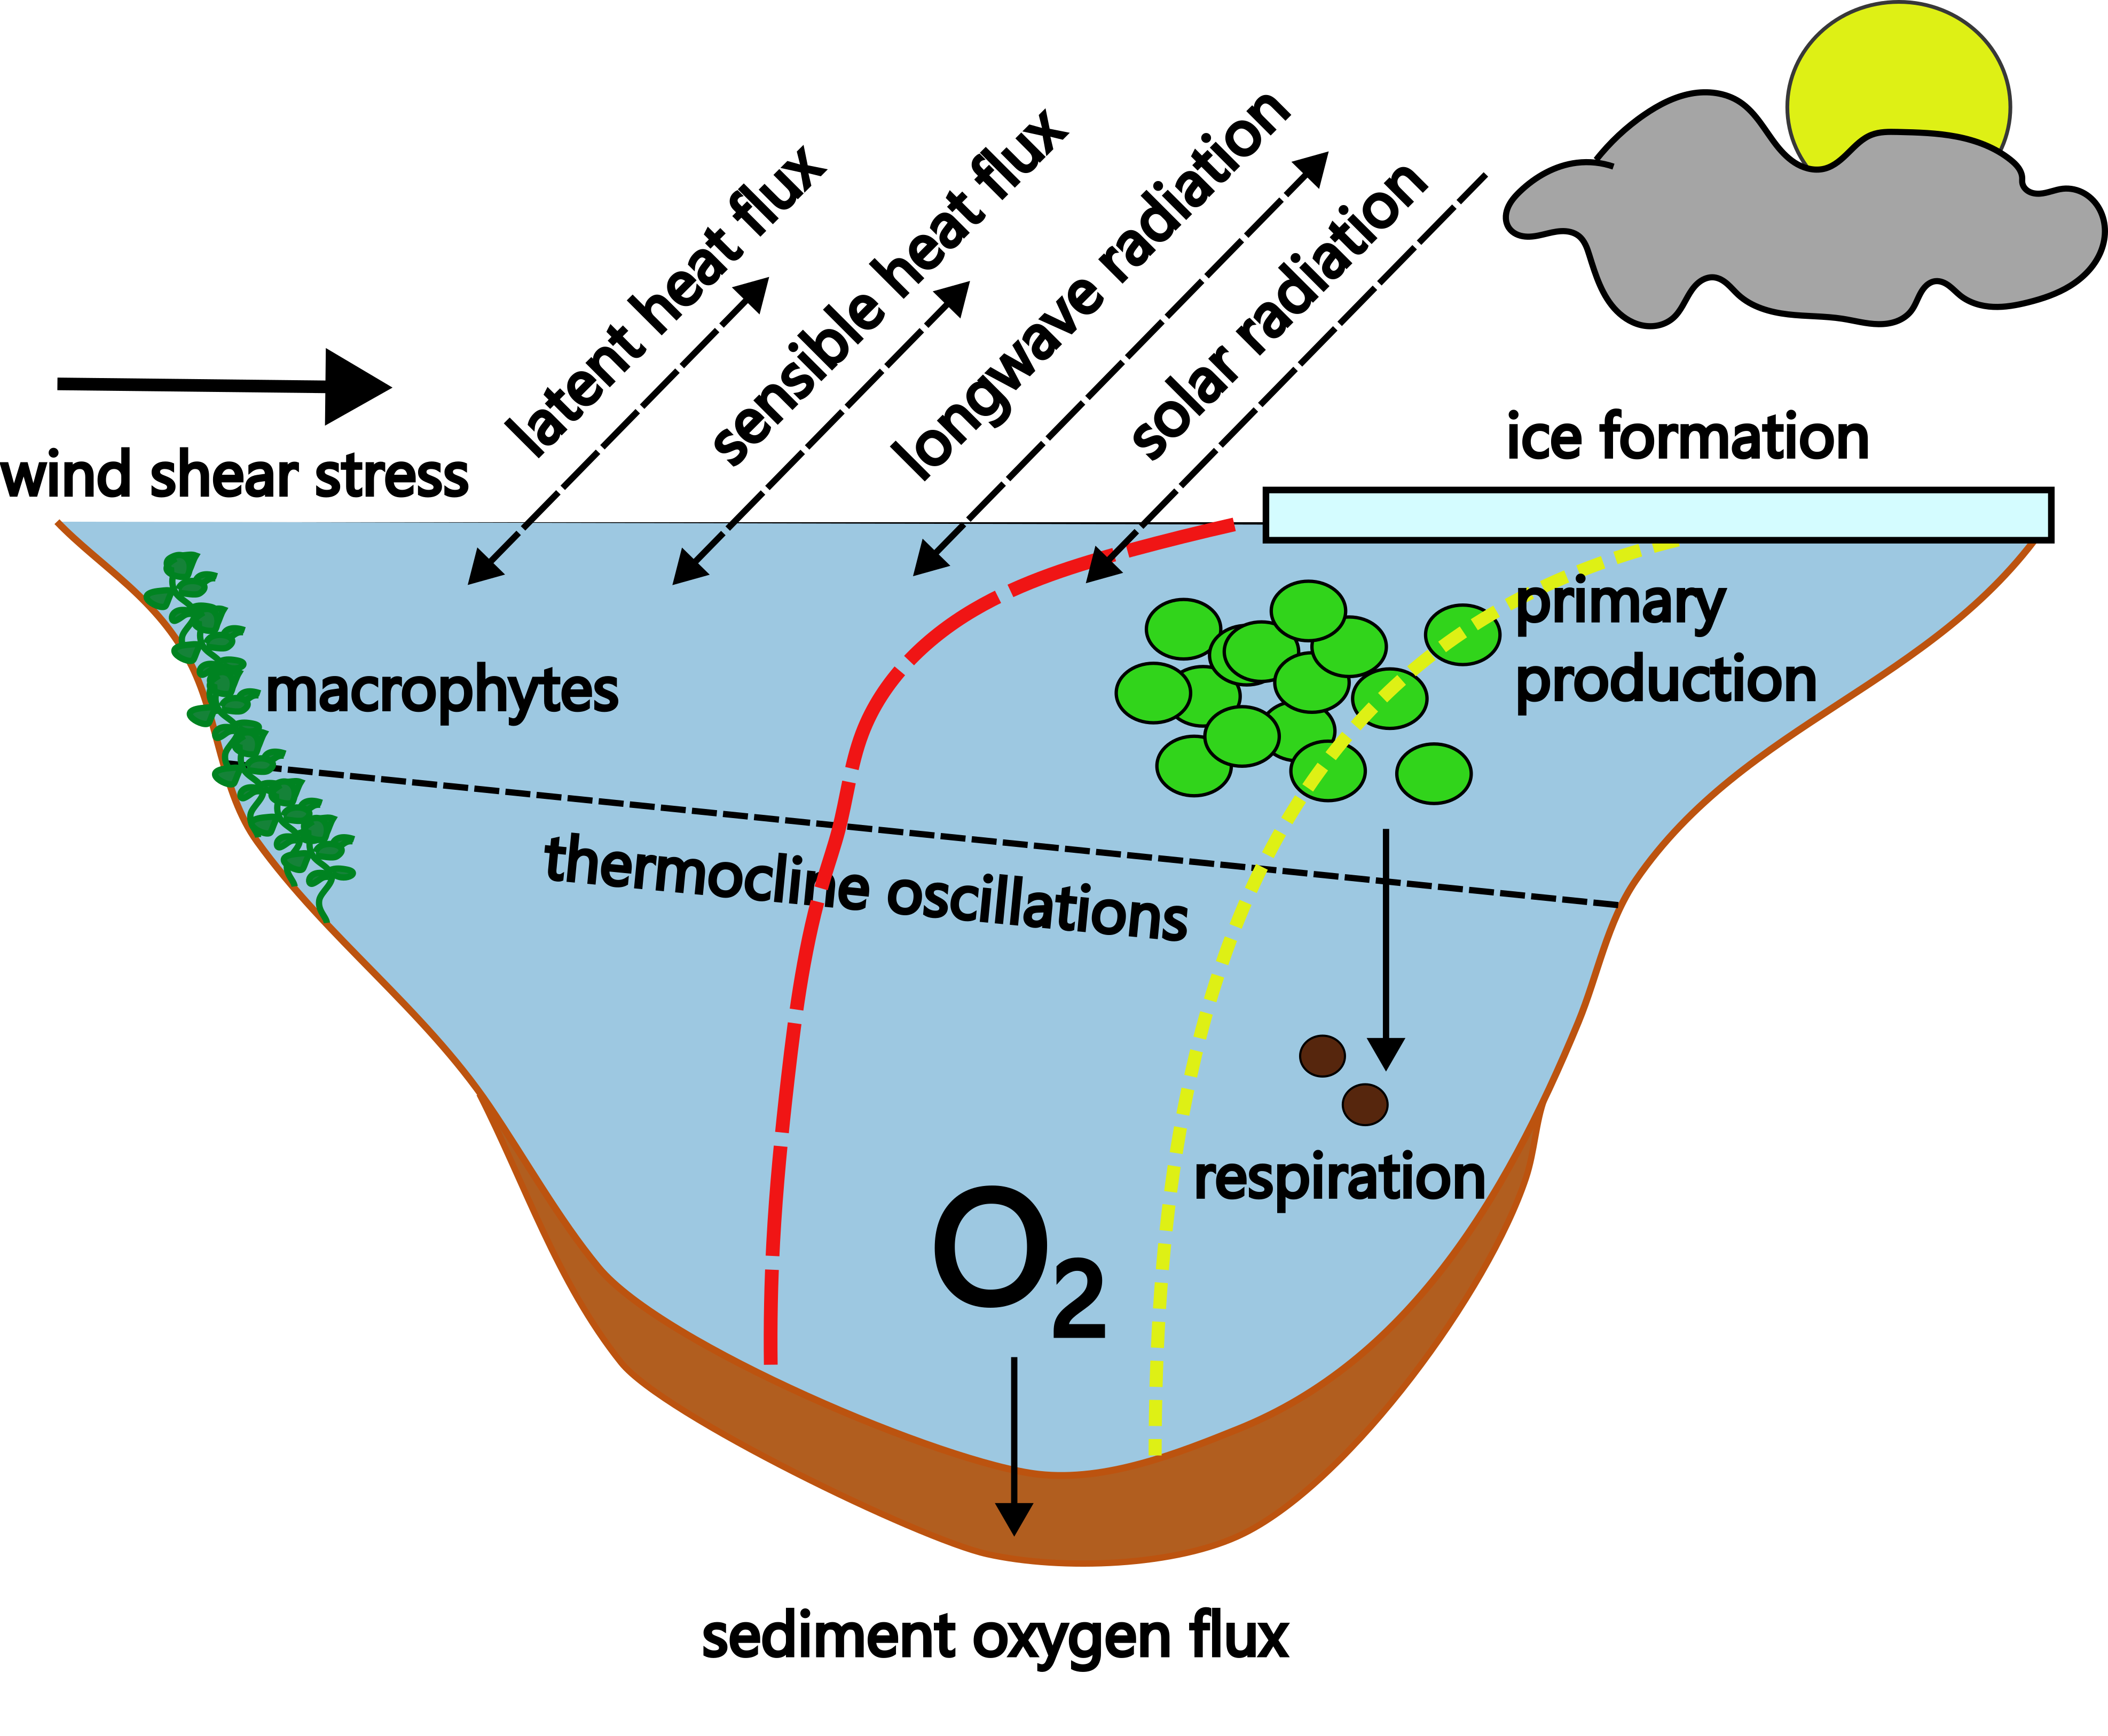
\includegraphics{graphics/LakeModelR_conceptart.png}
  \caption{Lake stratification.  Source: \url{https://www.lakeaccess.org/lake-ecology/stratification}}
\end{figure}


href{https://portal.edirepository.org/nis/mapbrowse?scope=knb-lter-ntl&identifier=1&revision=60}{North Temperate Lakes LTER: Chemical Limnology of Primary Study Lakes: Nutrients, pH and Carbon 1981 - current}


\begin{knitrout}
\definecolor{shadecolor}{rgb}{0.969, 0.969, 0.969}\color{fgcolor}\begin{kframe}
\begin{alltt}
\hlcom{# Model lake stratification using LakeR}

\hlcom{# Load the LakeModelR package}
\hlkwd{library}\hlstd{(}\hlstr{"LakeModelR"}\hlstd{)}
\end{alltt}
\end{kframe}
\end{knitrout}


\subsection{Modeling Lake Temperatures}

\begin{knitrout}
\definecolor{shadecolor}{rgb}{0.969, 0.969, 0.969}\color{fgcolor}\begin{kframe}


{\ttfamily\noindent\itshape\color{messagecolor}{\#\# Loading required package: tidyverse}}

{\ttfamily\noindent\itshape\color{messagecolor}{\#\# -- Attaching packages --------------------------------------- tidyverse 1.3.2 --\\\#\# v ggplot2 3.3.6 \ \ \ \ v purrr \ \ 1.0.2\\\#\# v tibble \ 3.2.1 \ \ \ \ v dplyr \ \ 1.1.4\\\#\# v tidyr \ \ 1.2.0 \ \ \ \ v stringr 1.5.1\\\#\# v readr \ \ 2.1.2 \ \ \ \ v forcats 0.5.2\\\#\# -- Conflicts ------------------------------------------ tidyverse\_conflicts() --\\\#\# x dplyr::filter() masks stats::filter()\\\#\# x dplyr::lag() \ \ \ masks stats::lag()\\\#\# Joining with `by = join\_by(dt)`\\\#\# Joining with `by = join\_by(dt, datetime, Shortwave\_Radiation\_Downwelling\_wattPerMeterSquared, Longwave\_Radiation\_Downwelling\_wattPerMeterSquared, Air\_Temperature\_celsius, Relative\_Humidity\_percent, Ten\_Meter\_Elevation\_Wind\_Speed\_meterPerSecond, Precipitation\_millimeterPerDay, Snowfall\_millimeterPerDay, Surface\_Level\_Barometric\_Pressure\_pascal, date, Cloud\_Cover, ea)`}}

{\ttfamily\noindent\color{warningcolor}{\#\# Warning in initial\_profile(initfile = system.file("{}extdata"{}, "{}observedTemp.txt"{}, : Meteorological starting date is 2009-01-01, but observed data starts 20 days later on 2009-01-21}}\begin{verbatim}
## What a beautiful day to run a lake model.================================================================================Time difference of 30.83752 secs
## Have a lovely rest of your day!
\end{verbatim}
\end{kframe}
\end{knitrout}

\begin{knitrout}
\definecolor{shadecolor}{rgb}{0.969, 0.969, 0.969}\color{fgcolor}
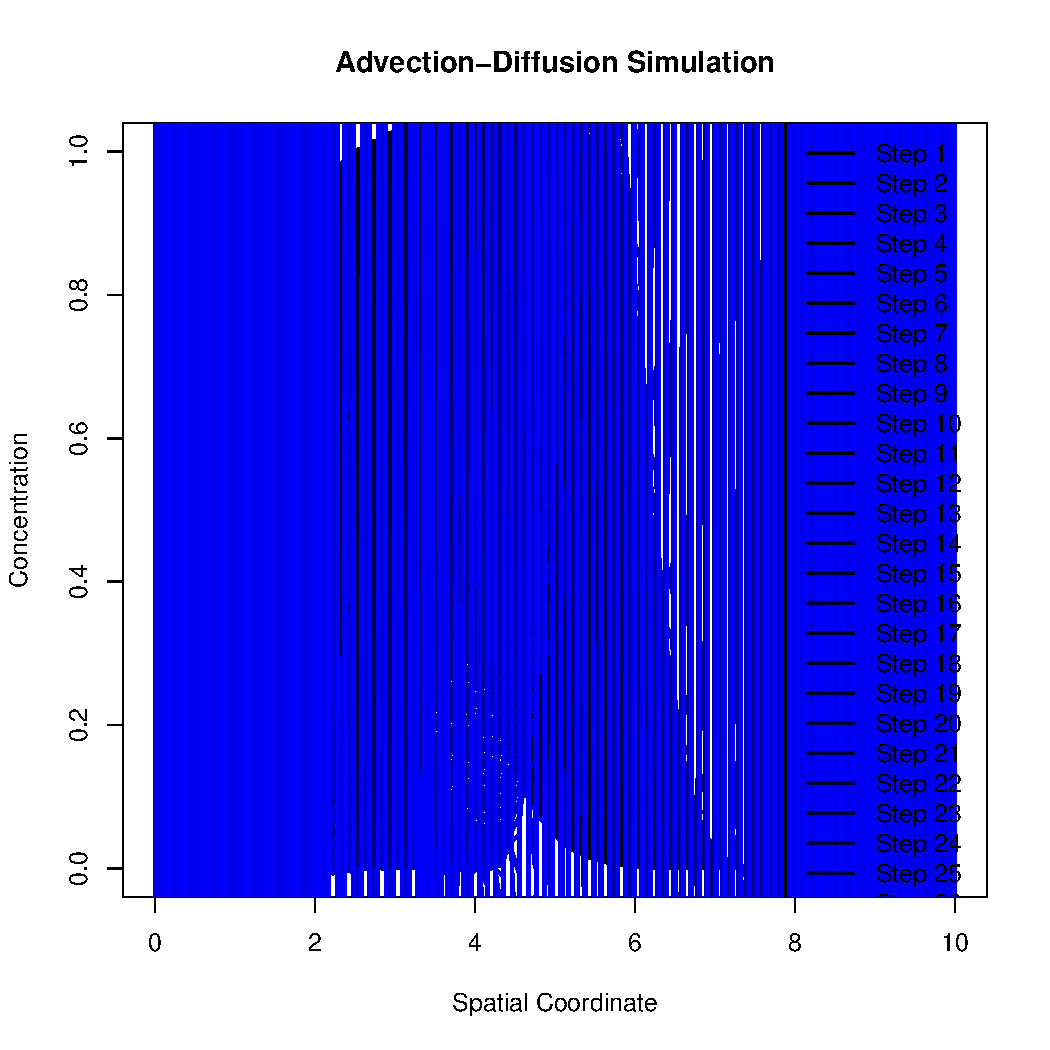
\includegraphics[width=\maxwidth]{figure/unnamed-chunk-3-1} 
\end{knitrout}


\begin{knitrout}
\definecolor{shadecolor}{rgb}{0.969, 0.969, 0.969}\color{fgcolor}
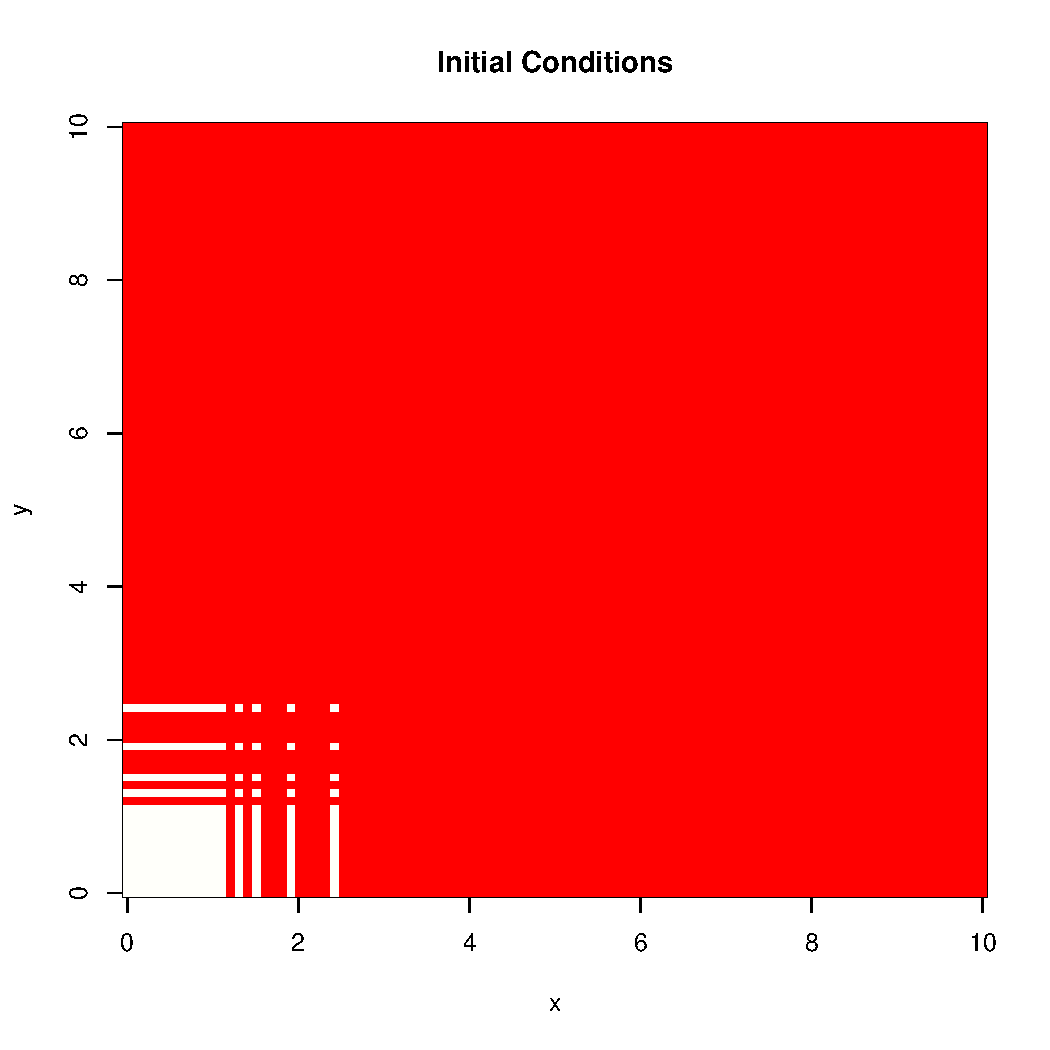
\includegraphics[width=\maxwidth]{figure/unnamed-chunk-4-1} 
\end{knitrout}





\subsection{Lake Mixing}



\begin{knitrout}
\definecolor{shadecolor}{rgb}{0.969, 0.969, 0.969}\color{fgcolor}\begin{kframe}
\begin{alltt}
\hlcom{# Model Oxygen Concentrations in Water}

\hlcom{# Parameters}
\hlstd{temperature} \hlkwb{<-} \hlkwd{seq}\hlstd{(}\hlnum{0}\hlstd{,} \hlnum{30}\hlstd{,} \hlkwc{by} \hlstd{=} \hlnum{1}\hlstd{)}  \hlcom{# Temperature in degrees Celsius}
\hlstd{bod} \hlkwb{<-} \hlkwd{seq}\hlstd{(}\hlnum{1}\hlstd{,} \hlnum{10}\hlstd{,} \hlkwc{by} \hlstd{=} \hlnum{1}\hlstd{)}  \hlcom{# Biological Oxygen Demand (BOD) in mg/L}
\hlstd{salinity} \hlkwb{<-} \hlkwd{seq}\hlstd{(}\hlnum{0}\hlstd{,} \hlnum{30}\hlstd{,} \hlkwc{by} \hlstd{=} \hlnum{1}\hlstd{)}  \hlcom{# Salinity in ppt (parts per thousand)}

\hlcom{# Model coefficients (example values, replace with actual coefficients)}
\hlstd{coeff_temp} \hlkwb{<-} \hlnum{0.5}
\hlstd{coeff_bod} \hlkwb{<-} \hlopt{-}\hlnum{0.2}
\hlstd{coeff_salinity} \hlkwb{<-} \hlopt{-}\hlnum{0.1}
\hlstd{intercept} \hlkwb{<-} \hlnum{10}

\hlcom{# Function to model oxygen concentration}
\hlstd{model_oxygen_concentration} \hlkwb{<-} \hlkwa{function}\hlstd{(}\hlkwc{temp}\hlstd{,} \hlkwc{bod}\hlstd{,} \hlkwc{salinity}\hlstd{) \{}
  \hlkwd{return}\hlstd{(intercept} \hlopt{+} \hlstd{coeff_temp} \hlopt{*} \hlstd{temp} \hlopt{+} \hlstd{coeff_bod} \hlopt{*} \hlstd{bod} \hlopt{+} \hlstd{coeff_salinity} \hlopt{*} \hlstd{salinity)}
\hlstd{\}}

\hlcom{# Generate a grid of combinations of temperature, BOD, and salinity}
\hlstd{grid} \hlkwb{<-} \hlkwd{expand.grid}\hlstd{(}\hlkwc{temperature} \hlstd{= temperature,} \hlkwc{bod} \hlstd{= bod,} \hlkwc{salinity} \hlstd{= salinity)}

\hlcom{# Model oxygen concentration for each combination}
\hlstd{grid}\hlopt{$}\hlstd{oxygen_concentration} \hlkwb{<-} \hlkwd{model_oxygen_concentration}\hlstd{(grid}\hlopt{$}\hlstd{temperature, grid}\hlopt{$}\hlstd{bod, grid}\hlopt{$}\hlstd{salinity)}

\hlcom{# Plotting the results}
\hlkwd{library}\hlstd{(}\hlstr{"scatterplot3d"}\hlstd{)}

\hlkwd{scatterplot3d}\hlstd{(grid}\hlopt{$}\hlstd{temperature, grid}\hlopt{$}\hlstd{bod, grid}\hlopt{$}\hlstd{salinity,} \hlkwc{color} \hlstd{=} \hlstr{"blue"}\hlstd{,}
              \hlkwc{main} \hlstd{=} \hlstr{"Oxygen Concentration Model"}\hlstd{,}
              \hlkwc{xlab} \hlstd{=} \hlstr{"Temperature (Celsius)"}\hlstd{,}
              \hlkwc{ylab} \hlstd{=} \hlstr{"BOD (mg/L)"}\hlstd{,}
              \hlkwc{zlab} \hlstd{=} \hlstr{"Salinity (ppt)"}\hlstd{,}
              \hlkwc{pch} \hlstd{=} \hlnum{16}\hlstd{,}
              \hlkwc{type} \hlstd{=} \hlstr{"h"}\hlstd{)}
\end{alltt}
\end{kframe}
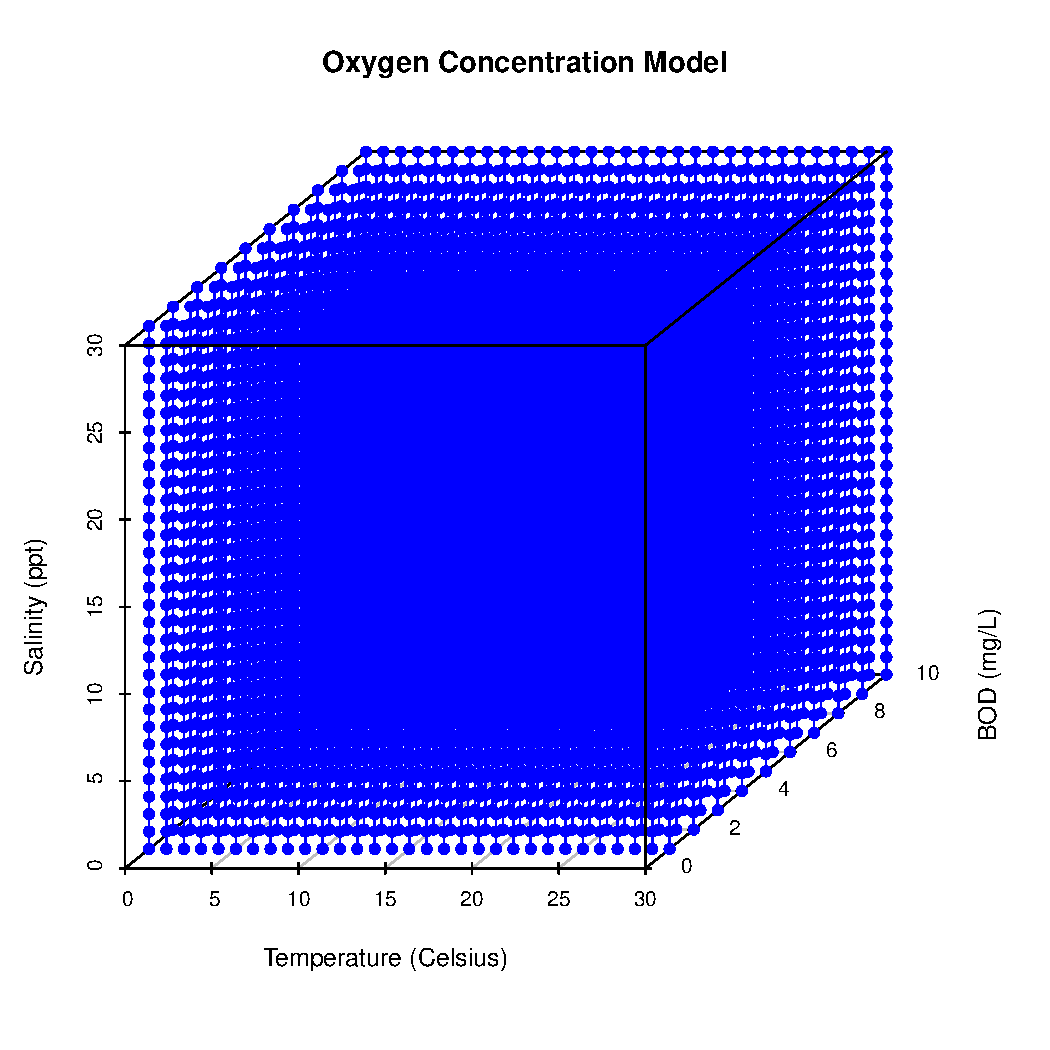
\includegraphics[width=\maxwidth]{figure/unnamed-chunk-7-1} 
\begin{kframe}\begin{alltt}
\hlcom{# Add model surface}
\hlstd{fit} \hlkwb{<-} \hlkwd{lm}\hlstd{(oxygen_concentration} \hlopt{~} \hlstd{temperature} \hlopt{+} \hlstd{bod} \hlopt{+} \hlstd{salinity,} \hlkwc{data} \hlstd{= grid)}
\hlstd{fit_surface} \hlkwb{<-} \hlkwd{predict}\hlstd{(fit,} \hlkwc{newdata} \hlstd{= grid)}
\hlkwd{scatterplot3d}\hlstd{(grid}\hlopt{$}\hlstd{temperature, grid}\hlopt{$}\hlstd{bod, grid}\hlopt{$}\hlstd{salinity,} \hlkwc{color} \hlstd{=} \hlstr{"blue"}\hlstd{,} \hlkwc{add} \hlstd{=} \hlnum{TRUE}\hlstd{,}
              \hlkwc{grid} \hlstd{=} \hlnum{FALSE}\hlstd{,} \hlkwc{fit} \hlstd{= fit_surface)}
\end{alltt}


{\ttfamily\noindent\color{warningcolor}{\#\# Warning in title(main, sub, ...): "{}add"{} is not a graphical parameter}}

{\ttfamily\noindent\color{warningcolor}{\#\# Warning in title(main, sub, ...): "{}fit"{} is not a graphical parameter}}

{\ttfamily\noindent\color{warningcolor}{\#\# Warning in plot.xy(xy.coords(x, y), type = type, ...): "{}add"{} is not a graphical parameter}}

{\ttfamily\noindent\color{warningcolor}{\#\# Warning in plot.xy(xy.coords(x, y), type = type, ...): "{}fit"{} is not a graphical parameter}}\end{kframe}
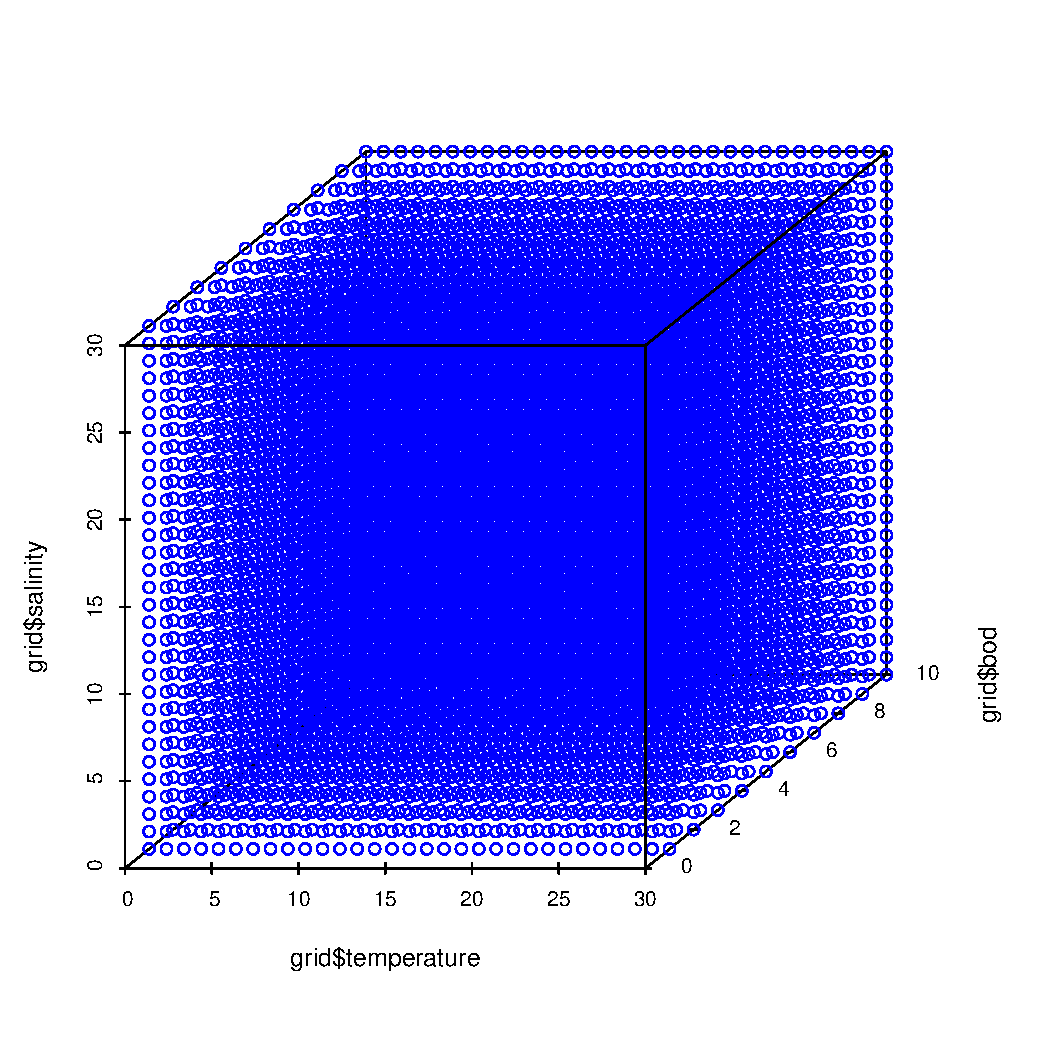
\includegraphics[width=\maxwidth]{figure/unnamed-chunk-7-2} 
\end{knitrout}


\end{document}
